% Physics experiment report
% 29/Oct/2016

\documentclass[a4paper,10pt,notitlepage]{article}

\usepackage{CJKutf8}
\usepackage{amsmath}
\usepackage{indentfirst}
\usepackage{graphicx}

\setlength{\parindent}{2em} 

\begin{CJK*}{UTF8}{gbsn}
\begin{document}

\title{测量媒质中的声速}
\author{秦光辉\ 9组3号}
\maketitle

\section{实验数据}

\subsection{极值法测空气中声速}

	第一组实验数据见表一.其中电压测量的最小分度为0.02V,x测量的最小分度为0.01mm.频率为
	
\begin{equation}
	f = 40.05000 kHz
\end{equation}

\begin{table}[htbp]
\centering

	\begin{tabular}{|c|c|c|c|c|c|}
	\hline
	$x_{i}$/mm & 39.214 & 43.619 & 47.918 & 52.065 & 56.442 \\
	\hline
	$V_{ppi}$/V & 3.72 & 3.20 & 3.00 & 2.68 & 2.40 \\
	\hline
	$x_{i+5}$/mm & 60.947 & 65.213 & 69.388 & 73.757 & 78.056 \\
	\hline
	$V_{pp i+5}$/V & 2.20 & 1.98 & 1.84 & 1.70 & 1.60 \\
	\hline
	$\Delta x_i$ & 21.733 & 21.594 & 21.470 & 21.692 & 21.614 \\
	\hline
	$\lambda$/mm & 8.6932 & 8.6376 & 8.5880 & 8.6768 & 8.6458 \\
	\hline
	\end{tabular}
	\caption{极值法正向测量数据表}

\end{table}

	计算上述$\lambda$的不确定度,有 
	
\begin{align}
	\bar{\lambda} &= 8.6483mm \\
	\sigma_{\bar{\lambda}} &= 0.02 mm \\
	\sigma_\lambda &= \sqrt{\sigma_{\bar{\lambda}} ^ 2 + (\frac{2e_x}{5\sqrt{3}})^2}  = 0.02mm \\
	\lambda \pm \Delta \lambda &= 8.65 \pm 0.02 mm
\end{align}

	信号发生器的精度非常高,近似认为其对实验误差贡献为0.则我们可以得到 
	
\begin{align}
	v_1 &= \lambda f = 346.3 m/s \\
	\sigma_{v_1} &= v_1 \times \frac{\sigma_{\lambda}}{\lambda} = 0.9 m/s \\
	v_1 \pm \Delta v_1 &= 346.3 \pm 0.9 m/s
\end{align}

	第二组实验数据见表二.其中电压测量的最小分度为0.02V,x测量的最小分度为0.01mm.频率为
	
\begin{equation}
	f = 40.05000 kHz
\end{equation}

\begin{table}[htbp]
\centering

	\begin{tabular}{|c|c|c|c|c|c|}
	\hline
	$x_{i}$/mm & 78.180 & 73.883 & 69.419 & 65.160 & 60.865 \\
	\hline
	$V_{ppi}$/V & 1.62 & 1.68 & 1.82 & 2.00 & 2.22 \\
	\hline
	$x_{i+5}$/mm & 56.534 & 52.161 & 47.821 & 43.533 & 39.116 \\
	\hline
	$V_{pp i+5}$/V & 2.42 & 2.70 & 3.00 & 3.18 & 3.66 \\
	\hline
	$\Delta x_i$ & 21.646 & 21.722 & 21.598 & 21.627 & 21.749 \\
	\hline
	$\lambda$/mm & 8.6584 & 8.6888 & 8.6392 & 8.6508 & 8.6996 \\
	\hline
	\end{tabular}
	\caption{极值法反向测量数据表}

\end{table}

	计算上述$\lambda$的不确定度,有 
	
\begin{align}
	\bar{\lambda} &= 8.6674mm \\
	\sigma_{\bar{\lambda}} &= 0.02 mm \\
	\sigma_\lambda &= \sqrt{\sigma_{\bar{\lambda}} ^ 2 + (\frac{2e_x}{5\sqrt{3}})^2}  = 0.02mm \\
	\lambda \pm \Delta \lambda &= 8.67 \pm 0.02 mm
\end{align}

	信号发生器的精度非常高,近似认为其对实验误差贡献为0.则我们可以得到 
	
\begin{align}
	v_2 &= \lambda f = 347.1 m/s \\
	\sigma_{v_2} &= v_2 \times \frac{\sigma_{\lambda}}{\lambda} = 1 m/s \\
	v_2 \pm \Delta v_2 &= 347 \pm 1 m/s
\end{align}

	综合上述两组数据,我们有
	
\begin{align}
	\bar{v} &= \frac{v_1 + v_2}{2} = 347 m/s \\
	\sigma_v &= \sqrt{(\frac{\sigma_{v_1}}{2})^2 + (\frac{\sigma_{v_2}}{2})^2} = 1 m/s \\
	v \pm \Delta v &= 347 \pm 1 m/s
\end{align}

\subsection{声音振幅随着距离的衰减图线}

	根据表一和表二的数据,我们可以做出图一和图二的曲线.从图线可以看出,声音随着距离呈指数式下降.
	
\begin{figure}[h]
	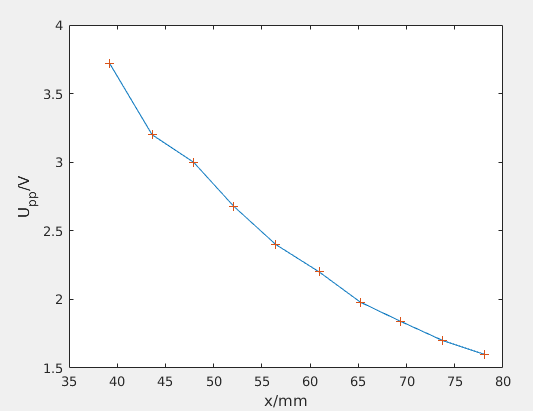
\includegraphics[scale=.6]{f1.png}
	\caption{声音振幅随x变化图线(正向测量值)}
\end{figure}
\begin{figure}[h]
	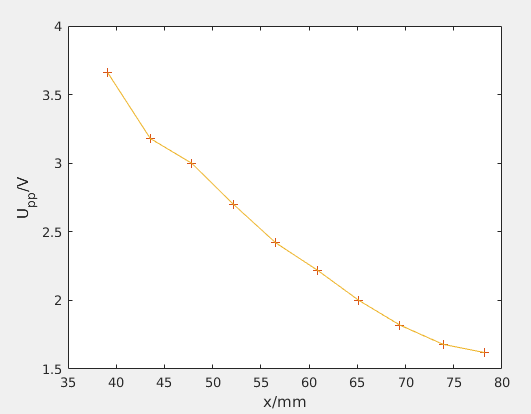
\includegraphics[scale=.6]{f2.png}
	\caption{声音振幅随x变化图线(反向测量值)}
\end{figure}

\subsection{相位法测空气中的声速}

	第三组实验数据见表三.其中电压测量的最小分度为0.02V,x测量的最小分度为0.01mm.频率为
	
\begin{equation}
	f = 40.05000 kHz
\end{equation}

\begin{table}[htbp]
\centering

	\begin{tabular}{|c|c|c|c|c|c|}
	\hline
	\# & 1 & 2 & 3 & 4 & 5 \\
	\hline
	$x_{i}$/mm & 32.729 & 41.417 & 50.069 & 58.328 & 67.154 \\
	\hline
	\# & 6 & 7 & 8 & 9 & 10 \\
	\hline
	$x_{i}$/mm & 75.811 & 84.232 & 93.013 & 101.425 & 110.054 \\
	\hline
	\end{tabular}
	\caption{相位法正向测量数据表}

\end{table}

	这样我们可以拟合直线,有
	
\begin{align}
	\lambda &= 8.5883mm \\
	b &= 24.19 mm \\
	r &= 1 - 7.92\times10^{-6}
\end{align}

	单个测量值的剩余方差为
	
\begin{align}
	\sigma ^ 2 = \frac{\sum_{i = 1}^{10}(x_i - b - n\lambda )^2}{10 - 2} = 0.009 mm^2 
\end{align}

	和仪器允差结合,有
	
\begin{align}
	\sigma_x = \sqrt{\sigma^2 + (\frac{e}{\sqrt{3}})^2} = 0.01 mm 
\end{align}

	斜率的不确定度为
	
\begin{align}
	\sigma_{\lambda} = \frac{\sigma_x}{\sqrt{\Sigma(n - \bar{n})^2}} = 0.02mm
\end{align}

	频率的精度很高,我们可以直接忽略频率对于实验误差的影响,可以得到:
	
\begin{align}
	v_1 &= \lambda f = 343.9 m/s \\
	\sigma_{v_1} &= v_1 * \frac{\sigma_{\lambda}}{\lambda} = 0.7m/s \\
	v_1 \pm \Delta v_1 &= 343.9 \pm 0.7m/s
\end{align}

	可以做出最小二乘法的图线如图三.
	
\begin{figure}[h]
	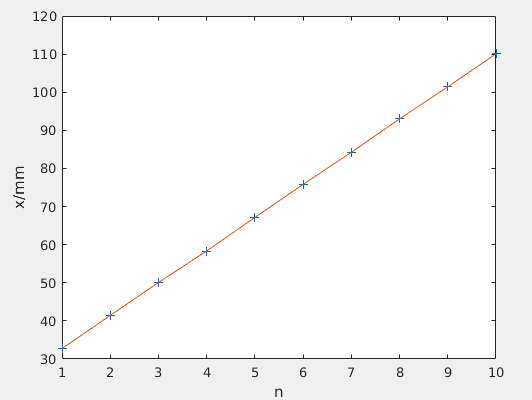
\includegraphics[scale=0.6]{f3.png}
	\caption{正向相位法测空气声速最小二乘法处理图线}
\end{figure}

	第四组实验数据见表三.其中电压测量的最小分度为0.02V,x测量的最小分度为0.01mm.频率为
	
\begin{equation}
	f = 40.05000 kHz
\end{equation}

\begin{table}[htbp]
\centering

	\begin{tabular}{|c|c|c|c|c|c|}
	\hline
	\# & 1 & 2 & 3 & 4 & 5 \\
	\hline
	$x_{i}$/mm & 110.018 & 101.345 & 93.903 & 84.132 & 75.603 \\
	\hline
	\# & 6 & 7 & 8 & 9 & 10 \\
	\hline
	$x_{i}$/mm & 67.064 & 58.232 & 50.035 & 41.300 & 32.589 \\
	\hline
	\end{tabular}
	\caption{相位法反向测量数据表}

\end{table}

	这样我们可以拟合直线,有
	
\begin{align}
	\lambda &= 8.6227mm \\
	b &= 118.84 mm \\
	r &= -1 + 9.21\times10^{-5}
\end{align}

	单个测量值的剩余方差为
	
\begin{align}
	\sigma ^ 2 = \frac{\sum_{i = 1}^{10}(x_i - b - n\lambda )^2}{10 - 2} = 0.012 mm^2 
\end{align}

	和仪器允差结合,有
	
\begin{align}
	\sigma_x = \sqrt{\sigma^2 + (\frac{e}{\sqrt{3}})^2} = 0.02 mm 
\end{align}

	斜率的不确定度为
	
\begin{align}
	\sigma_{\lambda} = \frac{\sigma_x}{\sqrt{\Sigma(n - \bar{n})^2}} = 0.03mm
\end{align}

	频率的精度很高,我们可以直接忽略频率对于实验误差的影响,可以得到:
	
\begin{align}
	v_2 &= \lambda f = 345.3 m/s \\
	\sigma_{v_2} &= v_2 * \frac{\sigma_{\lambda}}{\lambda} = 1m/s \\
	v_2 \pm \Delta v_2 &= 345 \pm 1m/s
\end{align}

	可以做出最小二乘法的图线如图四.
	
\begin{figure}[h]
	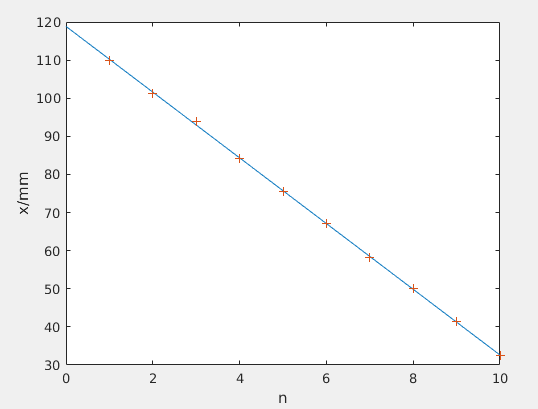
\includegraphics[scale=0.6]{f4.png}
	\caption{反向相位法测空气声速最小二乘法处理图线}
\end{figure}

	综合两组数据,有
	
\begin{align}
	\bar{v} &= \frac{v_1 + v_2}{2} = 344.6m/s \\
	\sigma_v &= \sqrt{(\frac{\sigma_{v_1}}{2})^2 + (\frac{\sigma_{v_2}}{2})^2} = 0.6 m/s \\
	v \pm \Delta v &= 344.6 \pm 0.6 m/s
\end{align}

\subsection{气体状态参量法}

	读得干温度计的读数为19.0$\pm 0.5 ^\circ$C,湿温度计度数为15.4$\pm 0.5 ^\circ$C(温度计最小分度值为1$^\circ$C).在湿度表上读得相应的湿度为68\%. \\
	
	由于温度计有示数上的误差,根据温度计上下限对应的湿度示数差值,粗略认为相对湿度的不确定度为5\%. \\
	
	表中读得19.0$^\circ$C下饱和蒸气压为2196.9Pa.考虑到温度计的读数误差,在18$^\circ$C和20$^\circ$C下饱和蒸气压为2063.6Pa和2337.8Pa,所以粗略估计其不确定度为
	
\begin{equation}
	\sigma_{p_w} = 100Pa.
\end{equation}

	这样我们可以计算空气中水蒸气的压强
	
\begin{align}
	p_w = 2.2 \pm 0.1 \times 10^3 Pa 
\end{align}
	
	气压计水银高度读数为752.20$\pm$0.05mm,我们可以获得空气的压强为
	
\begin{align}
	p &= 133.3224 \times h = 100285 Pa \\
	\sigma_p &= \frac{0.05}{\sqrt{3}} \times 133.3224 Pa = 4Pa
\end{align}

	代入书中的公式,我们有
	
\begin{align}
	v =& 343.6 m/s \\
	\sigma_v&=\sqrt{(\frac{\partial v}{\partial \theta}\sigma_\theta)^2+(\frac{\partial v}{\partial p_w}\sigma_{p_w})^2+(\frac{\partial v}{\partial p}\sigma_p)^2}=0.3m/s
\end{align}
	
	最终有
	
\begin{equation}
	v = 343.6 \pm 0.3 m/s
\end{equation}

\subsection{水中光栅测量水中声速}
	
	实验中卷尺的最小分度为0.1cm,测得光栅到墙壁的距离为468.0cm.频率的精度为0.1MHz,厘米尺的精度为0.1cm.我测了一组频率值下一级亮斑的间距,数据如表五.
	
\begin{table}[htbp]
\centering

	\begin{tabular}{|c|c|c|c|c|c|c|c|c|}
	\hline
	f/MHz & 10.38 & 10.85 & 11.23 & 11.41 & 11.76 & 12.09 & 12.29 & 12.68 \\
	\hline
	$\Delta x$/cm & 4.15 & 4.39 & 4.50 & 4.55 & 4.73 & 4.83 & 4.92 & 5.08 \\
	\hline
	\end{tabular}
	\caption{水中光栅测量数据表}

\end{table}

	由于衍射角非常小,我们近似得到以下公式.
	
\begin{equation}
	v = \frac{2fL\lambda}{\Delta x}
\end{equation}

	使用最小二乘法获得f和$\Delta x$的关系,得到
	
\begin{align}
	k &= 2.5225 MHz/cm \\
	b &= -0.127MHz \\
	r &= 0.99786 \\
	\sigma ^ 2 &= \frac{\sum_{i = 1}^{8}(f_i - b - kx_i )^2}{8 - 2} \\
	\sigma_f &= \sqrt{\sigma^2 + (\frac{e}{\sqrt{3}})^2} \\
	\sigma_{k} &= \frac{\sigma_f}{\sqrt{\Sigma(x_i - \bar{x})^2}} = 0.2 MHz/cm
\end{align}

	结合所有误差,有
	
\begin{align}
	v &= 1495 m/s \\
	\sigma_v &= \sqrt{\sigma_L ^ 2 + \sigma_{f/\Delta x} ^ 2} * v = 100 m/s \\
	v &= 1.5 \pm 0.1 \times 10^3 m/s
\end{align}

\subsection{极值法测水下声速}

	第三组实验数据见表六.x测量的最小分度为0.01mm.频率为
	
\begin{equation}
	f = 1.853000 MHz
\end{equation}

\begin{table}[htbp]
\centering

	\begin{tabular}{|c|c|c|c|}
	\hline
	$x_{i}$/mm & 33.033 & 33.402 & 33.817 \\
	\hline
	$x_{i+3}$/mm & 34.615 & 35.021 & 35.437 \\
	\hline
	$\Delta x_i$ & 1.582 & 1.619 & 1.62 \\
	\hline
	$\lambda$/mm & 0.791 & 0.810 & 0.810 \\
	\hline
	\end{tabular}
	\caption{极值法正向测量水下声速数据表}

\end{table}

	计算上述$\lambda$的不确定度,有 
	
\begin{align}
	\bar{\lambda} &= 0.804mm \\
	\sigma_{\bar{\lambda}} &= 0.006mm \\
	\sigma_\lambda &= \sqrt{\sigma_{\bar{\lambda}} ^ 2 + (\frac{e_x}{4\sqrt{3}})^2}  = 0.01mm \\
	\lambda \pm \Delta \lambda &= 0.80 \pm 0.01 mm
\end{align}

	信号发生器的精度非常高,近似认为其对实验误差贡献为0.则我们可以得到 
	
\begin{align}
	v_1 &= \lambda f = 1.48 \times 10^3 m/s \\
	\sigma_{v_1} &= v_1 \times \frac{\sigma_{\lambda}}{\lambda} = 20 m/s \\
	v_1 \pm \Delta v_1 &= 1.48 \pm 0.02  m/s
\end{align}

	第四组实验数据见表八.其中电压测量的最小分度为0.02V,x测量的最小分度为0.01mm.频率为
	
\begin{equation}
	f = 1.853000 MHz
\end{equation}

\begin{table}[htbp]
\centering

	\begin{tabular}{|c|c|c|c|}
	\hline
	$x_{i}$/mm & 35.319 & 34.998 & 34.600 \\
	\hline
	$x_{i+3}$/mm & 33.772 & 33.399 & 32.975 \\
	\hline
	$\Delta x_i$ & 1.547 & 1.599 & 1.625 \\
	\hline
	$\lambda$/mm & 0.774 & 0.780 & 0.813 \\
	\hline
	\end{tabular}
	\caption{极值法测水下声速反向测量数据表}

\end{table}

	计算上述$\lambda$的不确定度,有 
	
\begin{align}
	\bar{\lambda} &= 0.800mm \\
	\sigma_{\bar{\lambda}} &= 0.01 mm \\
	\sigma_\lambda &= \sqrt{\sigma_{\bar{\lambda}} ^ 2 + (\frac{2e_x}{5\sqrt{3}})^2}  = 0.02mm \\
	\lambda \pm \Delta \lambda &= 0.80 \pm 0.02 mm
\end{align}

	信号发生器的精度非常高,近似认为其对实验误差贡献为0.则我们可以得到 
	
\begin{align}
	v_2 &= \lambda f = 1.48 \times 10^3 \\
	\sigma_{v_2} &= v_2 \times \frac{\sigma_{\lambda}}{\lambda} = 30 m/s \\
	v_2 \pm \Delta v_2 &= 1.46 \pm 0.03 \times 10^3 m/s
\end{align}

	综合上述两组数据,我们有
	
\begin{align}
	\bar{v} &= \frac{v_1 + v_2}{2} = 1.48 \times 10^3 m/s \\
	\sigma_v &= \sqrt{(\frac{\sigma_{v_1}}{2})^2 + (\frac{\sigma_{v_2}}{2})^2} = 20 m/s \\
	v \pm \Delta v &= 1.48 \pm 0.02 \times 10^3 m/s
\end{align}

\subsection{相位法测量水下声速}

	第三组实验数据见表八.x测量的最小分度为0.01mm.频率为
	
\begin{equation}
	f = 1.853000 MHz
\end{equation}

\begin{table}[htbp]
\centering

	\begin{tabular}{|c|c|c|c|c|c|c|c|c|}
	\hline
	\# & 1 & 2 & 3 & 4 & 5 & 6 & 7 & 8 \\
	\hline
	$x_{i}$/mm & 35.875 & 36.698 & 37.471 & 38.285 & 39.113 & 39.877 & 40.633 & 41.476 \\
	\hline
	\end{tabular}
	\caption{相位法正向测量水下声速数据表}

\end{table}

	这样我们可以拟合直线,有
	
\begin{align}
	\lambda &= 0.79676mm \\
	b &= 35.093 mm \\
	r &= 0.99993
\end{align}

	单个测量值的剩余方差为
	
\begin{align}
	\sigma ^ 2 = \frac{\sum_{i = 1}^{10}(x_i - b - n\lambda )^2}{10 - 2} = 0.01 mm^2 
\end{align}

	和仪器允差结合,有
	
\begin{align}
	\sigma_x = \sqrt{\sigma^2 + (\frac{e}{\sqrt{3}})^2} = 0.02 mm 
\end{align}

	斜率的不确定度为
	
\begin{align}
	\sigma_{\lambda} = \frac{\sigma_x}{\sqrt{\Sigma(n - \bar{n})^2}} = 0.02mm
\end{align}

	频率的精度很高,我们可以直接忽略频率对于实验误差的影响,可以得到:
	
\begin{align}
	v_1 &= \lambda f = 1.48 \times 10^3 m/s \\
	\sigma_{v_1} &= v_1 * \frac{\sigma_{\lambda}}{\lambda} = 10m/s \\
	v_1 \pm \Delta v_1 &= 1.48 \pm 0.01 \times 10^3 m/s
\end{align}

	可以做出最小二乘法的图线如图五. \\
	
\begin{figure}[h]
	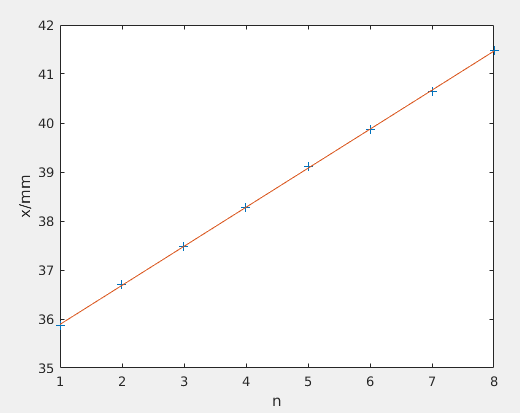
\includegraphics[scale=0.6]{f5.png}
	\caption{正向相位法测水中声速最小二乘法处理图线}
\end{figure}

	第四组实验数据见表九.其中电压测量的最小分度为0.02V,x测量的最小分度为0.01mm.频率为
	
\begin{equation}
	f = 1.853000 MHz
\end{equation}

\begin{table}[htbp]
\centering

	\begin{tabular}{|c|c|c|c|c|c|c|c|c|}
	\hline
	\# & 1 & 2 & 3 & 4 & 5 & 6 & 7 & 8 \\
	\hline
	$x_{i}$/mm & 41.333 & 40.592 & 39.786 & 39.001 & 38.211 & 37.421 & 36.632 & 35.827 \\
	\hline
	\end{tabular}
	\caption{相位法测水下声速反向测量数据表}

\end{table}

	这样我们可以拟合直线,有
	
\begin{align}
	\lambda &= 0.7884mm \\
	b &= 42.184 mm \\
	r &= -0.99997
\end{align}

	单个测量值的剩余方差为
	
\begin{align}
	\sigma ^ 2 = \frac{\sum_{i = 1}^{10}(x_i - b - n\lambda )^2}{10 - 2} = 0.01 mm^2 
\end{align}

	和仪器允差结合,有
	
\begin{align}
	\sigma_x = \sqrt{\sigma^2 + (\frac{e}{\sqrt{3}})^2} = 0.02 mm 
\end{align}

	斜率的不确定度为
	
\begin{align}
	\sigma_{\lambda} = \frac{\sigma_x}{\sqrt{\Sigma(n - \bar{n})^2}} = 0.02mm
\end{align}

	频率的精度很高,我们可以直接忽略频率对于实验误差的影响,可以得到:
	
\begin{align}
	v_2 &= \lambda f = 1.46 \times 10^3 m/s \\
	\sigma_{v_2} &= v_2 * \frac{\sigma_{\lambda}}{\lambda} = 20 m/s \\
	v_2 \pm \Delta v_2 &= 1.46 \pm 0.02 \times 10^3 m/s 
\end{align}

	可以做出最小二乘法的图线如图六.
	
\begin{figure}[h]
	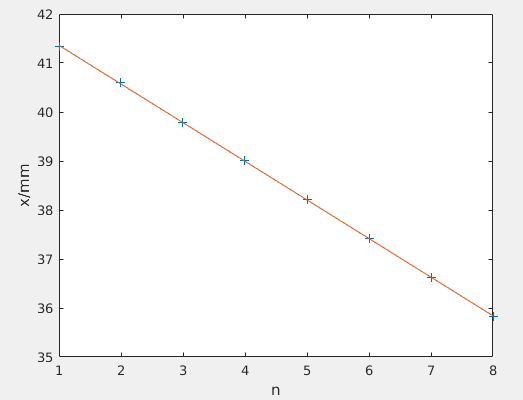
\includegraphics[scale=0.6]{f6.png}
	\caption{反向相位法测水中声速最小二乘法处理图线}
\end{figure}

	综合两组数据,有
	
\begin{align}
	\bar{v} &= \frac{v_1 + v_2}{2} = 1.47 \times 10^3 m/s \\
	\sigma_v &= \sqrt{(\frac{\sigma_{v_1}}{2})^2 + (\frac{\sigma_{v_2}}{2})^2} = 20 m/s \\
	v \pm \Delta v &= 1.47 \pm 0.02 \times 10^3 m/s 
\end{align}

\section{讨论和分析}

	在极值法和相位法实验中,误差最大的因素是对于换能器位置的确定.极值法中难以判断什么时候到达峰值,利萨如图形也很难保持直线,由于各种扰动,图线总是在不停跳动.极值法我尝试在每次到达峰值之后开始下降的一瞬间记录数据,这样虽然正向和反向数据有所不同,但是每个数据都记录的相对准确.相位法中我尽可能放大利萨如图形,可以减小一定误差. \\
	
	回程差是一个非常大的干扰因素,但是可以通过向前拨动转轮再向后拨来消除. \\
	
	气体状态参量法中,温度和湿度的测量非常不精准.这是最大的误差项.相对而言,湿度的影响更大一些. \\
	
	光栅实验中,最大的误差项来自于光斑间距的测定.由于只能在墙上测定,而且光路不一定和墙面垂直,只有厘米尺可以测定,所以实验非常困难.但是可以通过最小二乘法尽可能减小误差. \\
	
	极值法和相位法的水下声速测量实验中,误差非常大.主要来自于无法固定换能器和外界干扰太多,导致图线非常不稳定.而且如果换能器没有对准,图线非常粗,不好判断极值和相位.这是最大的误差项. \\
	
	但是三项声速测定实验的五个声速数据都比较接近,可见不确定因素虽然多,误差虽然大,但还是可以测到一个相对合力的声速值的.

\section{思考题}

\subsection{ }

	波长是个很小的数值,随机误差比较大.多次测量可以减小随机误差. \\
	
	在处理数据时,逐差法比首尾相减再取平均更好.首尾相减再相加的方法会把中间的数据浪费.而逐差法利用了更多的数据.
	
\subsection{ }

	相位法之中,振幅最大是图像特征最明显,便于测量.利萨如图形中呈直线的时候图线最为明显,所以在直线时记录数据,误差最小.

\end{CJK*}
\end{document}
